
%(BEGIN_QUESTION)
% Copyright 2012, Tony R. Kuphaldt, released under the Creative Commons Attribution License (v 1.0)
% This means you may do almost anything with this work of mine, so long as you give me proper credit

The following diagrams show windings for different {\it two-speed} induction AC motors, along with connection instructions for each of the operating speeds:

$$\includegraphics[width=15.5cm]{i02137x01.eps}$$

Identify the ``wye'' or ``delta'' configurations for each of these motors, in each of their speeds.

\vskip 10pt

Also, explain the principle behind the two speeds of each motor.  Hint: the ``low speed'' configuration runs at half the speed as the ``high speed'' configuration.

\vskip 20pt \vbox{\hrule \hbox{\strut \vrule{} {\bf Suggestions for Socratic discussion} \vrule} \hrule}

\begin{itemize}
\item{} A helpful problem-solving technique to apply in this case is to mark the coils with polarity (+,$-$) symbols as if they were being energized by DC, in order to better picture how the coils in each pair relate to each other.
\end{itemize}

\underbar{file i02137}
%(END_QUESTION)





%(BEGIN_ANSWER)

The left-hand motor always operates in a ``wye'' configuration.  The right-hand motor operates as a ``delta'' in the low-speed mode and as a ``wye'' in the high-speed mode.

\vskip 10pt

These motors achieve half-speed operation by doubling the number of active poles in their stators.  Note that in each of the high-speed configurations, pairs of stator coils are connected in parallel so that they act as one coil.  In each of the low-speed configurations, stator coils are connected in series with opposing polarities, so that they will have opposite magnetic poles and therefore function differently.

The doubling of poles is not unlike a doubling of light bulbs in a ``chaser'' light display, where the sequential blinking of light bulbs gives them an appearance of motion.  Adding more light bulbs in between the existing bulbs of a chaser array (i.e. doubling the number of lights without changing the length of the array) makes it appear as though the lights' ``motion'' moves along at a slower pace for the same blinking frequency.

%(END_ANSWER)





%(BEGIN_NOTES)


%INDEX% Pictorial circuit review (3-phase motor connections)

%(END_NOTES)


